\documentclass[tikz,margin=2mm]{standalone}
\pagestyle{empty}

%\usepackage{aistats2020}
\usepackage{amsmath}
\usepackage{bm}
\usetikzlibrary{positioning,calc,arrows,arrows.meta}

\begin{document}

	% PC algorithm MI test 400 samples
	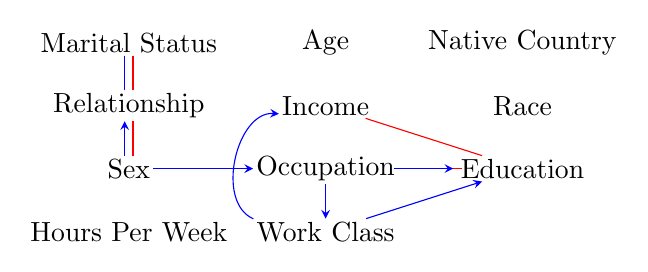
\begin{tikzpicture}
	\begin{scope}[xscale=1, yscale=1]
		\tikzstyle{every node}=[align=center, inner sep=1pt]
		\node (ms)   at (0, 0)    {\textrm{Marital Status}};
		\node (rln)  at (0, -0.8) {\textrm{Relationship}};
		\node (sex)  at (0, -1.6) {\textrm{Sex}};
		\node (hrpw) at (0, -2.4) {\textrm{Hours Per Week}};

		\node (age) at (2.5, 0)    {\textrm{Age}};
		\node (inc) at (2.5, -0.8) {\textrm{Income}};
		\node (occ) at (2.5, -1.6) {\textrm{Occupation}};
		\node (wc)  at (2.5, -2.4) {\textrm{Work Class}};

		\node (nc)   at (5, 0)    {\textrm{Native Country}};
		\node (race) at (5, -0.8) {\textrm{Race}};
		\node (edu)  at (5, -1.6) {\textrm{Education}};

		\draw [red, transform canvas={xshift=0.15em}] (ms) to (rln);
		\draw [blue, transform canvas={xshift=-0.15em} ] (ms) to (rln);
		
		\draw [red, transform canvas={xshift=0.15em}] (rln) to (sex);
		\draw [blue, ->, >=stealth, transform canvas={xshift=-0.15em}] (sex) to (rln);

		\draw [red, transform canvas={xshift=0.15em}] (occ) to (edu);
		\draw [blue, ->, >=stealth, transform canvas={xshift=-0.15em}] (occ) to (edu);


		\draw [red] (inc) to (edu);

		\draw [blue, ->, >=stealth] (sex) to (occ);
		\draw [blue, ->, >=stealth] (occ) to (wc);
		\draw [blue, ->, >=stealth] (wc) to (edu);
		\draw [blue, ->, >=stealth] (wc) to[bend left=80] (inc);
	\end{scope}
	\end{tikzpicture}

	% PC algorithm Q3 test 400 samples
	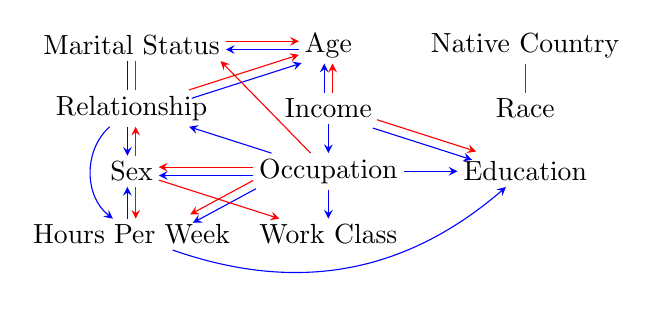
\begin{tikzpicture}
	\begin{scope}
		\tikzstyle{every node}=[align=center, inner sep=0.2em]
		\node (ms)   at (0, 0)    {\textrm{Marital Status}};
		\node (rln)  at (0, -0.8) {\textrm{Relationship}};
		\node (sex)  at (0, -1.6) {\textrm{Sex}};
		\node (hrpw) at (0, -2.4) {\textrm{Hours Per Week}};

		\node (age) at (2.5, 0)    {\textrm{Age}};
		\node (inc) at (2.5, -0.8) {\textrm{Income}};
		\node (occ) at (2.5, -1.6) {\textrm{Occupation}};
		\node (wc)  at (2.5, -2.4) {\textrm{Work Class}};

		\node (nc)   at (5, 0)    {\textrm{Native Country}};
		\node (race) at (5, -0.8) {\textrm{Race}};
		\node (edu)  at (5, -1.6) {\textrm{Education}};


		\draw [red, transform canvas={xshift=0.15em}] (ms) to (rln);
		\draw [blue, transform canvas={xshift=-0.15em}] (ms) to (rln);

		\draw [red, ->, >=stealth, transform canvas={xshift=0.15em}] (sex) to (rln);
		\draw [blue,->, >=stealth, transform canvas={xshift=-0.15em}] (rln) to (sex);		

		\draw [red, ->, >=stealth, transform canvas={xshift=0.15em}] (sex) to (hrpw);
		\draw [blue,->, >=stealth, transform canvas={xshift=-0.15em}] (hrpw) to (sex);

		\draw [red, ->, >=stealth, transform canvas={yshift=0.15em}] (ms) to (age);
		\draw [blue,->, >=stealth, transform canvas={yshift=-0.15em}] (age) to (ms);

		\draw [red, ->, >=stealth, transform canvas={yshift=0em}] (rln) to (age);
		\draw [blue,->, >=stealth, transform canvas={yshift=-0.3em, xshift=0.1em}] (rln) to (age);

		\draw [red, ->, >=stealth, transform canvas={xshift=0.15em}] (inc) to (age);
		\draw [blue,->, >=stealth, transform canvas={xshift=-0.15em}] (inc) to (age);
		\draw [red, ->, >=stealth, transform canvas={yshift=0.15em}] (inc) to (edu);
		\draw [blue,->, >=stealth, transform canvas={xshift=-0.15em, yshift=-0.15em}] (inc) to (edu);

		\draw [red, ->, >=stealth, transform canvas={yshift=0.15em}] (occ.-170) to (hrpw.15);
		\draw [blue,->, >=stealth, transform canvas={yshift=-0.15em, xshift=0.1em}] (occ.-170) to (hrpw.15);
		
		\draw [red, ->, >=stealth, transform canvas={yshift=0.15em}] (occ) to (sex);
		\draw [blue,->, >=stealth, transform canvas={yshift=-0.15em}] (occ) to (sex);
		
		
		\draw [red, ->, >=stealth] (sex) to (wc);
		\draw [red, ->, >=stealth] (occ) to (ms.-10);
		\draw [red] (nc) to (race);

		\draw [blue,->, >=stealth] (rln) to[bend right=50] (hrpw);
		\draw [blue,->, >=stealth] (hrpw) to[bend right=30] (edu);
		
		\draw [blue,->, >=stealth] (inc) to (occ);
		\draw [blue,->, >=stealth] (occ) to (rln);
		\draw [blue,->, >=stealth] (occ) to (wc);
		\draw [blue,->, >=stealth] (occ) to (edu);

	\end{scope}
	\end{tikzpicture}

	% Hill Climb with BIC Score Q3 test 400 samples
	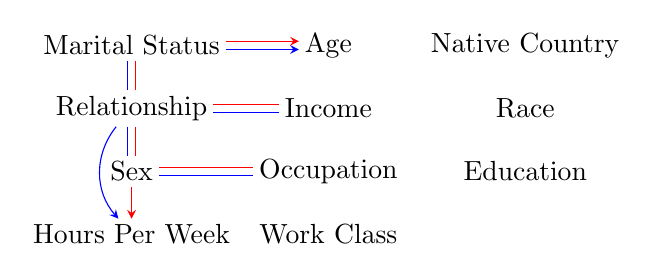
\begin{tikzpicture}
	\begin{scope}
		\tikzstyle{every node}=[align=center, inner sep=0.2em]

		\node (ms)   at (0, 0)    {\textrm{Marital Status}};
		\node (rln)  at (0, -0.8) {\textrm{Relationship}};
		\node (sex)  at (0, -1.6) {\textrm{Sex}};
		\node (hrpw) at (0, -2.4) {\textrm{Hours Per Week}};

		\node (age) at (2.5, 0)    {\textrm{Age}};
		\node (inc) at (2.5, -0.8) {\textrm{Income}};
		\node (occ) at (2.5, -1.6) {\textrm{Occupation}};
		\node (wc)  at (2.5, -2.4) {\textrm{Work Class}};

		\node (nc)   at (5, 0)    {\textrm{Native Country}};
		\node (race) at (5, -0.8) {\textrm{Race}};
		\node (edu)  at (5, -1.6) {\textrm{Education}};

		\draw [red, transform canvas={xshift=0.15em}] (ms) to (rln);
		\draw [blue, transform canvas={xshift=-0.15em}] (ms) to (rln);
		
		\draw [red, transform canvas={xshift=0.15em}] (rln) to (sex);
		\draw [blue, transform canvas={xshift=-0.15em}] (rln) to (sex);

		\draw [red, ->, >=stealth, transform canvas={yshift=0.15em}] (ms) to (age);
		\draw [blue, ->, >=stealth, transform canvas={yshift=-0.15em}] (ms) to (age);
		
		\draw [red, transform canvas={yshift=0.15em}] (rln) to (inc);
		\draw [blue, transform canvas={yshift=-0.15em}] (rln) to (inc);

		\draw [red, transform canvas={yshift=0.15em}] (sex) to (occ);
		\draw [blue, transform canvas={yshift=-0.15em}] (sex) to (occ);

		
		\draw [red, ->, >=stealth] (sex) to (hrpw);

		\draw [blue, ->, >=stealth] (rln) to[bend right=40] (hrpw);

	\end{scope}
	\end{tikzpicture}
\end{document}
